%% AVISO IMPORTANTE:
%% 
%% Este template es una versión modificada del template de la ACM sample-sigconf.tex.

\documentclass[sigconf]{acmart}

%% Datos del libro electrónico, a ser incluidos más adelante por los organizadores.
\setcopyright{rightsretained} %Uncomment this to keep your rights!
\setcopyright{CCBY} %Uncomment this to publish your work under Creative Commons!
\copyrightyear{2023}
\acmYear{2023}
\acmDOI{}

%% These commands are for a PROCEEDINGS abstract or paper.
\acmConference[]{TopTamaulipas 2023}{Noviembre, 2023}{Ciudad Victoria, TAMPS}
\acmBooktitle{}
\acmPrice{}
\acmISBN{XXXXXXXXXXXX}

\usepackage{subfigure}
\usepackage[utf8]{inputenc}
\usepackage[spanish]{babel}
%\usepackage[authoryear]{natbib}
%%

%% Inicio del cuerpo del artículo.
\begin{document}


%% "title" tiene un parámetro opcional, que le permite a los autores definir un título corto que aparece en los encabezados.
\title{Estrategias para la exploración coordinada multi-VANT}

%%
%% Los autores se inlcuyen usando el comando "author". El ejemplo muestra distintos casos, cuando hay autores que comparten afiliación o no.
%% "authornote" y "authornotemark" son usados para denotar contribuciones compartidas en la investigación, por los autores.
\author{Luis Alberto Ballado Aradias}
%\authornote{Nota.}
\email{luis.ballado@cinvestav.mx}
%\orcid{orcidxxxxxxxx}
%\authornotemark[1]
\affiliation{%
  \institution{Cinvestav Unidad Tamaulipas}
  \streetaddress{Parque Cient\'ifico y Tecnol\'ogico de Tamaulipas}
  \city{Victoria}
  \state{Tamps}
  \country{Mexico}
  \postcode{87138}
}

\author{Dr. José Gabriel Ramírez Torres}
\email{grtorres@cinvestav.mx}
\affiliation{%
  \institution{Cinvestav Unidad Tamaulipas}
  \streetaddress{Parque Cient\'ifico y Tecnol\'ogico de Tamaulipas}
  \city{Victoria}
  \state{Tamps}
  \country{Mexico}
  \postcode{87138}
}


\author{Dr. Eduardo A. Rodriguez Tello}
\email{ertello@cinvestav.mx}
\affiliation{%
  \institution{Cinvestav Unidad Tamaulipas}
  \streetaddress{Parque Cient\'ifico y Tecnol\'ogico de Tamaulipas}
  \city{Victoria}
  \state{Tamps}
  \country{Mexico}
  \postcode{87138}
}

%% Título en encabezado
\renewcommand{\shortauthors}{Ballado, et al.}
\renewcommand{\tablename}{Tabla}
%%
%% Resumen del trabajo que se está presentando.
\begin{abstract}

  Las estrategias de exploración son de suma importancia en esfuerzos como misiones de búsqueda y rescate, así como en el mapeo de zonas afectadas por desastres naturales. Los vehículos aéreos no tripulados (VANTS) han ganado una gran popularidad en estos escenarios debido a su movilidad, ya que cuentan con la capacidad de cubrir grandes áreas de interés. Con el avance de la electrónica a bordo de los VANTS, la investigación se ha desplazado hacia la toma de decisiones para misiones que involucran múltiples VANTS. No obstante, la navegación autónoma y la exploración de áreas extensas inexploradas siguen siendo un desafío, especialmente en ambientes cambiantes por obstáculos móviles.\\

  Un enfoque colaborativo ofrece mejores resultados de exploración con una rápida obtención de información, logrando sus objetivos con un alto grado de consistencia y resilencia a fallos en comparación con una implementación donde se emplea un único vehículo aéreo no tripulado. Sin embargo, la exploración multi-VANT plantea diversos desafíos que deben abordarse para su correcto funcionamiento, como la comunicación, la colaboración y la fusión de datos.\\
  
  Este trabajo presenta la propuesta de una arquitectura descentralizada de software capaz de coordinar múltiples VANTS con habilidades para la exploración, generación de mapas y planificación de rutas para explorar eficientemente un área de interés, garantizando la adaptabilidad a cambios en su entorno. Este problema implica la toma de decisiones complejas, como asignar tareas de exploración a los VANTS, evitar colisiones y planificar rutas óptimas. Factores como la comunicación entre VANTS, la incertidumbre del entorno y las limitaciones de recursos de energía forman parte de los criterios considerados.

  %Si se trata de un artículo de discusión, describa el tópico central a desarrollar y/o la problemática subyacente junto con la motivación para ser abordada desde la perspectiva de la investigación o el desarrollo tecnológico. Empleando un lenguaje accesible y claro para la mayor audiencia posible, describa de manera breve las principales aplicaciones e impacto que el tópico a tratar representa, desde la perspectiva de la sociedad.
\end{abstract}

%%
%% Keywords. Incluir no menos de tres palabas clave que identifiquen el trabajo presentado. Separar las palabras con coma.
\keywords{Estrategias multi-VANT, exploración multi-VANT, planificación de rutas multi-VANT}

%% Creación de la primera parte del documento formateado, incluyendo título y autores.
\maketitle

%% Primera sección del artículo
\section{Introducción}

Los robots de servicio son máquinas autónomas diseñadas con el objetivo de prestar servicio a los humanos fuera del ambiente industrial, convirtiéndose poco a poco en una parte esencial en nuestras vidas. Los podemos encontrar en diversos ámbitos, como en el entretenimiento, limpieza, logística, entre otras soluciones inovadoras \cite{INTEL2023}.\\

Los vehículos aéreos no tripulados han evolucionado rápidamente y se han convertido en sistemas versátiles capaces de una amplia gama de aplicaciones, desde vigilancia hasta misiones de búsqueda y rescate \cite{Schneider2016}. Entre ellas, las tareas de exploración en entornos complejos y dinámicos representan un área interesante y desafiante, donde la coordinación efectiva de múltiples VANT se vuelve primordial. Este tema es de creciente importancia a medida que los vehículos aéreos no tripulados continúan transformando distintas áreas, incluida la agricultura, el monitoreo ambiental, mantenimiento de infraestructuras (puentes, edificios, líneas eléctricas) y la respuesta a desastres naturales, reduciendo los riesgos y costos asociados con las inspecciones manuales.\\

Los VANTS capaces de realizar tareas con autonomía generalmente cuentan con mayores capacidades de carga y procesamiento computacional, así como sensores capaces de percibir grandes volúmenes de datos en un tiempo reducido. Estos VANTS se centran en realizar tareas sencillas y estáticas en áreas abiertas con rutas predeterminadas, o bien, en contextos de operación por control remoto por un usuario. Sin embargo en donde los espacios son estrechos, se optan por el uso de VANTS reducidos, comúnmente llamados Micro-Vehículos Aéreos no tripulados (MAVs).\\%Para aplicaciones complejas, donde se debe responder de manera autónoma con la mínima intervención humana, es decir, que solo se le ordene la tarea que deben realizar y no guiarlos en cada uno de sus movimientos.\\

Un sistema autónomo de un Vehículo Aéreo no Tripulado, consta de cuatro algoritmos:

\begin{itemize}
\item Generación de una representación del entorno
\item Planificación de trayectorias
\item Evasión de obstáculos
\item Comunicación
\end{itemize}

La computadora embebida para un sistema de navegación usado en Micro-Vehículos Aéreos son de bajo rendimiento, pero su necesidad de autonomía sigue siendo la misma que un VANT de mayor tamaño. Es por ello que es necesario equiparlos con algoritmos de baja complejidad computacional.\\

La necesidad de coordinación entre múltiples VANTS en tareas de exploración, surge debido a las limitaciones individuales en cuanto a la extensión de terreno que pueden cubrir y su desempeño. La exploración de áreas extensas o peligrosas a menudo exige un enfoque colaborativo, donde los VANTS trabajen juntos para optimizar la asignación de recursos y mejorar la recopilación y el análisis de datos.\\

Sin embargo, el camino hacia una coordinación entre múltiples vehículos aéreos no tripulados, presenta diversos desafíos. Las complejidades de gestionar un grupo de vehículos aéreos no tripulados, navegar en entornos dinámicos y distribuir tareas de forma inteligente son sólo algunas de las cuestiones que exigen nuestra atención. El objetivo del documento es explorar y proponer una estrategia para mejorar la coordinación de múltiples VANTS en el contexto de las tareas de exploración.\\

%En esta introducción, brindamos una descripción general de la importancia del tema, destacando la relevancia cada vez mayor de las misiones de exploración con múltiples vehículos aéreos no tripulados y las deficiencias de los métodos de coordinación existentes. También sentamos las bases para nuestras discusiones posteriores, que incluirán una revisión exhaustiva del estado actual del arte, una discusión de los objetivos de la investigación y un resumen de la estructura de este artículo.\\

La exploración de áreas desconocidas, a través de la sinergia de sistemas multi-VANT promete ser una solución innovadora. Al comprender y perfeccionar una estrategia para la coordinación de múltiples vehículos aéreos no tripulados en tareas de exploración, esperamos descubrir nuevas posibilidades, replicar o romper los límites existentes, y en última instancia, avanzar en los campos de la robótica y la exploración.\\

El presente trabajo de investigación busca resolver las siguientes preguntas de investigación:

\begin{itemize}
  \item ¿Cuáles son los principales desafíos que limitan la coordinación eficaz de múltiples vehículos aéreos no tripulados en tareas de exploración?
  \item ¿Cómo se pueden aprovechar desde sensores avanzados hasta algoritmos de inteligencia artificial, para superar estos desafíos?
  \item ¿Cuáles son las implicaciones de una mejor coordinación de múltiples vehículos aéreos no tripulados para diversos sectores, incluida la exploración autónoma en interiores?
\end{itemize}

Si bien este artículo no presenta resultados en esta etapa, sirve como una exploración de un dominio de investigación en evolución y guía para esfuerzos futuros en este campo. Al abordar estos desafíos y ampliar los límites de la tecnología de los vehículos aéreos no tripulados, nos esforzamos por conocer nuevas posibilidades para el descubrimiento científico, la gestión ambiental y los esfuerzos humanitarios.

%% Cuerpo principal, dividido por secciones.
\section{Trabajos Relacionados}

El despliegue rápido de robots en situaciones de riesgo, búsqueda y rescate ha sido un área ampliamente estudiada en la robótica móvil. Existen concursos como el DARPA Subterranean Challenge, donde los factores como la exploración, planeación y coordinación son clave para lograr los objetivos del reto \cite{DARPA2022}.\\

La dirección en que apunta el estado del arte, se puede atribuir a los avances en tecnología en la última década. Investigadores de diversas áreas, que incluyen las ciencias computacionales y la ingeniería, han contribuido al crecimiento de este campo.\\

Un enfoque ampliamente adoptado para estudiar la exploración en robótica implica la utilización de fronteras, que delinean los límites entre espacios conocidos y desconocidos. Estas fronteras sirven para identificar áreas potencialmente informativas, guiando eficientemente el proceso de exploración hasta que no se detecten más fronteras, lo que indica la conclusión de la exploración.\\

Sin embargo, si bien las metodologías basadas en fronteras han demostrado ser efectivas en términos de cobertura de área, a menudo dan como resultado movimientos subóptimos, particularmente cuando se aplican a vehículos aéreos no tripulados. La causa fundamental de esta ineficiencia puede atribuirse principalmente a las limitaciones de las tecnologías sensoriales utilizadas para construir mapas del medio ambiente con fines de exploración. Los sensores comunes equipados en vehículos aéreos no tripulados, como las cámaras RGB-D y sensores láser tipo LiDAR, tienen rangos de detección limitados. En consecuencia, los vehículos aéreos no tripulados se ven obligados a adoptar patrones de vuelo cautelosos para garantizar la seguridad.\\

\begin{figure}
    \centering
    \subfigure[]{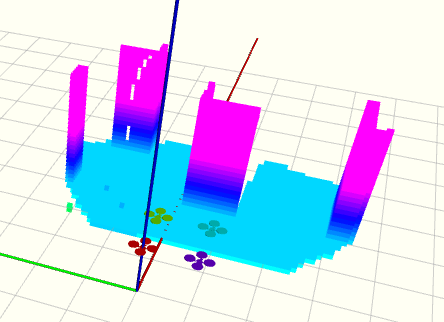
\includegraphics[width=0.23\textwidth]{racer_drone.png}} 
    \subfigure[]{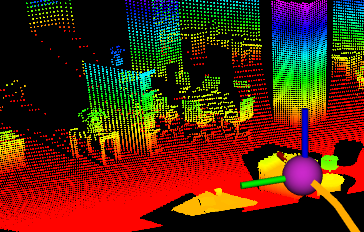
\includegraphics[width=0.23\textwidth]{aerial_navigation.png}}
    \caption{Una representación del ambiente, guiará a una mejor navegación autónoma. \\(a) RACER-Exploración multi-VANT Mapa global.\\ (b) Falco-Navegación \cite{Zhang2023} Autónoma mono-VANT Mapa para su navegación local.}
    \label{fig:foobar}
\end{figure}

Para abordar esta limitación, \citeauthor{CIESLEWSKI2017} \cite{CIESLEWSKI2017}, proponen una estrategia de exploración que genera directivas de velocidad basadas en fronteras recientemente identificadas, con el objetivo de maximizar la velocidad del VANT. Este enfoque demuestra un rendimiento superior en comparación con los métodos tradicionales, pero se centra exclusivamente en las fronteras locales.\\

Por el contrario, \citeauthor{FUEL} \cite{FUEL}, introducen un enfoque de planificación jerárquica que produce rutas globales eficientes al tiempo que promueve maniobras locales seguras y ágiles para la exploración. Sin embargo, esta estrategia requiere el mantenimiento de un historial de fronteras activas.\\

En la Figura \ref{fig:foobar}, se ilustra dos enfoques diferentes en una navegación autónoma. Por una parte (a), se tiene que una representación del mapa global compartido puede ayudar en un enfoque colaborativo. Por otro lado (b), una representación local beneficia en conocer los objetos a su paso.\\% Haciendo del sensado constante del ambiente una pieza fundamental en el ciclo de autonomía de un VANT.\\

En el ámbito de la mejora de la eficiencia de la exploración, se han introducido en la literatura científica varios métodos que implican la cooperación entre múltiples robots, presentados tanto en forma centralizada como descentralizada. Los métodos centralizados suelen incorporar una estación terrestre central responsable de calcular inicialmente un plan integral para múltiples robots, que luego se difunde a los agentes, suponiendo una comunicación fluida. En este sentido, \citeauthor{1435481} \cite{1435481}, se esfuerzan por reducir la superposición en áreas exploradas disminuyendo la ganancia de información de una frontera potencial si se asigna otro robot a una frontera separada en su proximidad. En cambio, \citeauthor{Tian} \cite{Tian}, abordan el desafío de la asignación utilizando un problema de vendedores ambulantes múltiples (mTSP por sus siglas en inglés) para asignar a cada agente a una frontera candidata. Mientras tanto, el enfoque propuesto por \citeauthor{9844235} \cite{9844235}, sobresale en generar caminos eficientes para la reconstrucción 3D. Sin embargo, es importante señalar que este método requiere un sobrevuelo previo del área de interés, lo que la hace inadecuada para la exploración donde no se tiene conocimiento previo del área de interés. Por otro lado, el método descrito por \citeauthor{Tian} \cite{Tian}, pone un mayor énfasis en la navegación a través de bosques, con un enfoque particular en la estimación y el mapeo colaborativos del estado, en lugar de la planificación de rutas.\\

No obstante, los sistemas centralizados, por diseño, operan bajo el supuesto de una comunicación confiable a larga distancia. Además, enfrentan desafíos relacionados con la escalabilidad, ya que la carga de trabajo de la unidad central de procesamiento aumenta con el creciente número de agentes. Por otro lado, los enfoques descentralizados son intrínsecamente más sólidos debido a que no tienen dependencia de comunicación directa. En estos métodos, cada robot puede funcionar independientemente de los demás, lo que ofrece una mayor resiliencia. Sin embargo, esta ventaja tiene el costo de una mayor complejidad en la coordinación de las acciones de los agentes, ya que se limitan a utilizar información local exclusivamente.\\

\citeauthor{YAMAUCHI1997} \cite{YAMAUCHI1997} presenta una estrategia en la que los robots se mueven hacia la frontera más cercana e intercambian datos de mapas con otros agentes. Sin embargo, este enfoque resulta ineficiente porque puede dar lugar a que varios robots converjan en la misma frontera. \citeauthor{9483227} \cite{9483227}, abordan esta limitación basando su enfoque en la teoría del transporte óptimo, mientras que \citeauthor{9561328} \cite{9561328}, emplean un campo potencial de múltiples objetivos y múltiples robots para la asignación a diferentes fronteras. Mientras que \citeauthor{9561226} \cite{9561226}, asignan robots a grupos de fronteras. Sin embargo, estos métodos se basan en el supuesto de una comunicación estable entre agentes.\\

El enfoque introducido por \citeauthor{RACER2022} \cite{RACER2022}, conocido como RACER, tiene como objetivo mitigar estos problemas dividiendo el área de exploración en una cuadrícula y garantizando que los agentes exploren distintas regiones mientras siguen rutas de cobertura. RACER es resistente ante rangos de comunicación limitados, ya que depende de la interacción directa por pares entre robots. Sin embargo, enfrenta desafíos en términos de coordinación subóptima en entornos muy concurridos, ya que supone una distribución uniforme de los obstáculos.\\

Dentro de los trabajos realizados en el Cinvestav Unidad Tamaulipas en el área de la exploración coordinada se encuentra el trabajo de \citeauthor{CINVESTAM2013} \cite{CINVESTAM2013}, donde propone una estrategia descentralizada para la exploración Multi-Robot con un enfoque en auto-ofertas considerando los robots como agentes económicos que buscan realizar el mejor aporte al proceso de exploración decidiendo en base a la situación actual, sin interferir con la misión de los demás robots.\\

Motivados por estas limitaciones, nuestra investigación introduce una estrategia descentralizada para sistemas de múltiples VANTS, que englobe los componentes necesarios para realizar tareas de exploración en interiores.

\section{Objetivos e Hipótesis}

\subsection*{Objetivo general}

Uno de los desafíos fundamentales que enfrentamos reside en la capacidad de coordinar múltiples VANT en tareas de exploración y mapeo.\\

En este contexto, el objetivo general es abordar y resolver este desafío, desarrollando una arquitectura de software descentralizada capaz de resolver los problemas de localización, mapeo, navegación y coordinación multi-VANT en ambientes desconocidos y dinámicos para tareas de exploración en interiores.

\subsection*{Objetivos Particulares}

En el marco de esta investigación, establecemos metas concretas que dirigen nuestro trabajo hacia el desarrollo de una estrategia destinada a optimizar la exploración coordinada de un grupo de vehículos aéreos no tripulados.\\

\begin{itemize}
\item Evaluar y comparar diferentes algoritmos de coordinación y planificación de vuelo para la exploración coordinada multi-VANT.
\item Elegir la representación del ambiente con menor complejidad computacional.
\item Realizar pruebas y simulaciones de la solución propuesta en entornos complejos, analizando métricas como tiempo de exploración, cobertura del área de interés y calidad de los datos recopilados.
\end{itemize}

\subsection*{Hipótesis}

Esta innovadora área de estudio se centra en la coordinación y colaboración de múltiples VANTS para llevar a cabo tareas de exploración y observación en entornos complejos. La hipótesis subyacente en este campo de investigación se fundamenta en la idea de la implementación de una estrategia de exploración coordinada utilizando múltiples vehículos aéreos no tripulados (multi-VANT) en entornos complejos, permitirá obtener mejores resultados en comparación con la exploración individual (mono-VANT). Esta coordinación eficiente se traducirá en una reducción del tiempo y los recursos necesarios para completar la exploración, así como en una mayor cobertura del área de interés. Además, se espera que la exploración coordinada multi-VANT mejore la calidad de los datos recopilados, lo que permitirá tomar decisiones más informadas y eficaces en diversos campos, como la cartografía, la vigilancia, el monitoreo y la respuesta a desastres naturales.

\section{Planteamiento del problema}

Dada un área de interés desconocida en un espacio cerrado que se desea explorar denotada como $\mathcal{A}$, tal que $\mathcal{A} \subset \mathbb{R}^{3}$.\\

Un voxel $v$ que representa el espacio contenido en $\mathcal{A}$ que es obtenido dividiendo recursivamente el área de interés $\mathcal{A}$ en ocho partes de igual tamaño, el voxel puede tomar los valores de libre, ocupado y desconocido o no explorado de notados como $v_{libre}$, $v_{ocup}$, $v_{desc}$. La región ocupada son obtenidas mediante un sensor basado en un modelo de ocupación probabilístico.\\

Un conjunto de VANTS denotado como $\mathcal{V} = \{\mathcal{V}_{1},\mathcal{V}_{2},\mathcal{V}_{3},...,\mathcal{V}_{n}\}$ siendo $n$ el número total de VANTS disponibles y una configuración inicial $q$ cuya cardinalidad es el número de VANTS disponibles denotado como $q = \{q_{1},q_{2},q_{3},...,q_{n}\}$.\\

%Determinar el conjunto de tareas para cada VANT, así como el conjunto de rutas que maximize el área explorada minimizando el tiempo y la energía consumida.\\

La estrategia propuesta debe tomar en cuenta las limitaciones de comunicación, sensores y energía, para distribuir las tareas de exploración entre todos los miembros del equipo de VANTS, así como establecer trayectorias seguras y libres de obstáculos para cada uno de los VANTS.\\

Para lograr una exploraci\'{o}n eficiente y completa con un tiempo y recursos m\'{i}nimos, el problema requiere la creaci\'{o}n de algoritmos y t\'{e}cnicas de optimizaci\'{o}n.\\

La funci\'{o}n objetivo tomar\'{a} en cuenta distintos objetivos espec\'{i}ficos del problema:
\begin{itemize}
\item Maximizar la cobertura del \'{a}rea explorada 
\item Minimizar el tiempo total requerido para cubrir el \'{a}rea de inter\'{e}s
\item Asegurar la consistencia de la información recolectada y fusionada en un único mapa, compartido entre todos los VANTS
\end{itemize}

\section{Metodología}

Siguiendo los objetivos anteriores, la metodolog\'{i}a propuesta se divide en tres etapas, que comenzaron en septiembre del 2023 y terminarán en agosto de 2024. A continuaci\'{o}n se detallan cada una de las actividades que se plantean realizar en cada etapa.

\subsection*{Etapa 1. An\'{a}lisis y dise\~{n}o de la soluci\'{o}n propuesta}

Esta etapa comprende la revisi\'{o}n de la literatura de manera m\'{a}s completa, que permita contar con la informaci\'{o}n necesaria para la elecci\'{o}n de los mejores algoritmos para abordar cada una de las problem\'{a}ticas asociadas con la coordinaci\'{o}n de múltiples robots en tareas de exploración, detectando áreas de oportunidad para el desarrollo de una estrategia descentralizada de coordinación. 

\subsection*{Etapa 2. Implementaci\'{o}n y validaci\'{o}n}
  
  Esta etapa se centra en el desarrollo e implementaci\'{o}n del dise\~{n}o de la arquitectura de software para la coordinaci\'{o}n multi-VANT, utilizando una herramienta de simulación de robots de libre acceso, cumpliendo estándares de modularidad de diseño.
  
  \subsection*{Etapa 3. Evaluaci\'{o}n experimental, resultados y conclusiones}
  
  Partiendo del prototipo y las simulaciones desarrolladas en la etapa anterior, en esta etapa se realizan todas las actividades relacionadas con la evaluación, compilación y análisis de los resultados.
  
  
\section{Algoritmos}

Desarrollar una arquitectura para múltiples robots implica establecer un plan de toma de decisiones y definir un marco de interacción entre los distintos robots, lo cual afecta la configuración de cada robot individual, en donde las interacciones entre robots pueden tener lugar en diferentes niveles.\\

Un VANT cuenta con cuatro acuadores que generan movimientos en seis grados de libertad en posición y orientación. Esto significa que el VANT puede moverse en el espacio en cualquier dirección (adelante, atrás, izquierda, derecha, arriba, abajo) y rotar en todas las direcciones (girar sobre su eje longitudinal, lateral y vertical).\\
Cada rotor puede ajustar su velocidad para controlar su posición y orientación del VANT en todo momento. Al contar con un sistema sub-actuado (no puede controlar cada grado de libertad de manera independiente), se hacen uso de sistemas de control  que ajustan las velocidades de los rotores de manera inteligente para lograr los movimientos deseados.

\begin{figure}[h]
\centering
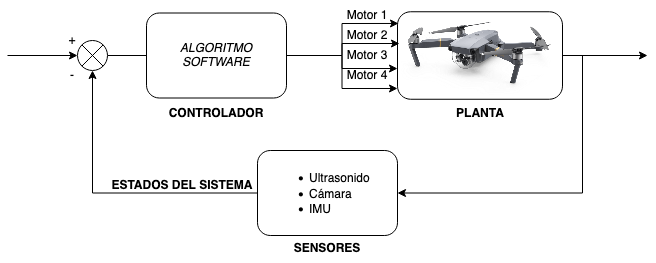
\includegraphics[width=0.5\textwidth]{control_drone}
\caption{Diagrama a bloques control de vuelo. \\La inteligencia emergente se realiza con la interacción constante de los sensores y estados actuales del VANT. Siendo estos un ciclo repetitivo a lo largo de la exploración.}
\label{fig:bloque}
\end{figure}

La autonomía de vuelo puede realizarse combinando el control de vuelo con la planificación de trayectorias y evasión de obstáculos. En sistemas autónomos como el ilustrado en la Figura \ref{fig:bloque}, la toma de decisiones determinará las instrucciones de vuelo en base a un objetivo. Los comandos son ejecutados haciendo que la aeronave siga la trayectoria calculada. El control de la planificación de movimiento se encarga de vincular los bucles interior y exterior de un sistema de vuelo autónomo y refleja la inteligencia del sistema.\\

Hay que considerar que el sistema de vuelo autónomo debe ejecutarse en línea, es decir en la tarjeta interna del VANT, para así lograr actualizar los estados del VANT y la información del mundo exterior.

\subsection*{Planificación de trayectorias}

La planificación de trayectorias para múltiples VANTS implica diseñar algoritmos y estrategias que permitan a cada VANT determinar la ruta óptima para cumplir con los objetivos de la misión, maximizando la eficiencia en términos de tiempo y recursos. Existen diferentes tipos de planificadores de trayectorias que se utilizan en el contexto de múltiples VANTS.

\begin{itemize}
  
\item Planificadores basados en algoritmos de búsqueda: Estos planificadores utilizan algoritmos de búsqueda clásicos, como A* \cite{Astar}, RRT \cite{RRT} o RRT* \cite{RRTstar}, para generar trayectorias seguras y óptimas para cada VANT.

\item Planificadores basados en optimización \cite{UAVOpt}: Estos planificadores plantean la generación de trayectorias como un problema de optimización, donde se busca encontrar la mejor trayectoria según criterios como minimizar el tiempo de vuelo, reducir el consumo de energía o maximizar la cobertura del área de interés.
  
\item Planificadores basados en aprendizaje por refuerzo \cite{DRL}: En este enfoque, se utilizan algoritmos de aprendizaje por refuerzo para enseñar a los VANTS a seleccionar las acciones adecuadas para alcanzar los objetivos de la misión. A través de la interacción con el entorno y la retroalimentación de recompensas, los VANTS mejoran su capacidad de planificación de trayectorias de forma autónoma.

\item Planificadores basados en enjambres [\citenum{Bio1},\citenum{Bio2},\citenum{Bio3}]: Estos planificadores se inspiran en los comportamientos observados en la naturaleza, como el vuelo en formación de las aves o el comportamiento de enjambre de las abejas. Mediante la coordinación y el seguimiento de patrones de vuelo predefinidos, los VANTS evitan colisiones y logran un rendimiento colectivo eficiente.
  
\end{itemize}

\subsection*{Mapeo}

La generación de mapas en 3D juega un papel fundamental en la navegación autónoma, permitiendo su desplazamiento seguro y eficiente en entornos complejos. Mediante el uso de sensores como lidar y cámaras, los VANTS capturan datos detallados del entorno, lo que les permite realizar una reconstrucción tridimensional precisa. Estos datos tridimensionales son utilizados para crear mapas que representan la estructura y los obstáculos del entorno en tiempo real. La construcción de mapas 3D para la navegación autónoma de VANTS implica técnicas avanzadas de procesamiento de datos y algoritmos sofisticados que fusionan y clasifican la información capturada por los sensores, generando una representación confiable y precisa del entorno tridimensional. Existen diversas técnicas empleadas en la generación de mapas en el ámbito de la robótica y la navegación autónoma.

\begin{itemize}

\item Mapeo basado en cuadrículas (grid-based mapping) \cite{GridUAV}: Esta aproximación divide el espacio del entorno en cuadrículas y asigna a cada celda un valor, indicando si está ocupada o libre. Los algoritmos de mapeo basado en cuadrículas, como Occupancy Grid Mapping, actualizan y mantienen un mapa de ocupación en tiempo real utilizando mediciones de los sensores para determinar la ocupación de las celdas.

\item Mapeo basado en características (feature-based mapping) \cite{LandmarksUAV}: Esta estrategia se basa en la detección y seguimiento de características distintivas (landmarks) del entorno, como esquinas o características visuales. Los algoritmos de mapeo basado en características emplean técnicas de extracción y emparejamiento de características para construir y actualizar un mapa basado en la ubicación y descripción de estas características.

\item Diagrama de Voronoi \cite{DVoronoi}: El diagrama de Voronoi es una estructura matemática que divide el espacio en regiones basadas en la proximidad a un conjunto de puntos de referencia. Los algoritmos de mapeo basados en el diagrama de Voronoi utilizan esta estructura para representar el entorno y facilitar la navegación a través de la información sobre la geometría del diagrama.

\item Mapeo basado en octree \cite{Octree2023}: Esta técnica divide el espacio del entorno en una estructura jerárquica de octantes tridimensionales. Cada octante puede ser etiquetado como ocupado o libre, permitiendo así una representación eficiente y detalladas.
\end{itemize}

\subsection*{Evasión de obstáculos}

La capacidad de esquivar obstáculos desempeña un papel fundamental en la navegación autónoma, ya que les permite evitar colisiones y mantener un vuelo seguro. Al contar con un VANT equipado con una variedad de sensores como lidar y cámaras, que les permiten detectar y comprender el entorno en tiempo real. Mediante el uso de algoritmos de detección y seguimiento de objetos, los VANTS pueden identificar diferentes obstáculos, desde edificios hasta árboles o personas. Utilizando esta información, los algoritmos de evasión de obstáculos analizan y determinan rutas seguras y viables para evitar los obstáculos detectados. Estos algoritmos emplean técnicas avanzadas de planificación de movimientos y toman decisiones rápidas y precisas para modificar la trayectoria del VANT y asegurar una navegación fluida. Existen diversos algoritmos empleados para evitar obstáculos en VANTS.

\begin{itemize}
\item Algoritmos de respuesta reactiva \cite{ReactiveCA}: Estos algoritmos se basan en la detección en tiempo real de obstáculos y generan maniobras de evasión de manera reactiva. Utilizan sensores y técnicas de percepción del entorno para identificar obstáculos y calcular trayectorias alternativas que eviten cualquier colisión.
\item Algoritmos de planificación de ruta \cite{ACA}: Estos algoritmos planifican trayectorias de vuelo que evitan áreas con obstáculos conocidos o detectados. Utilizan técnicas de planificación de caminos y buscan rutas seguras y eficientes basándose en los datos del entorno y los objetivos de navegación.
\item Algoritmos de aprendizaje automático \cite{AACA}: Estos algoritmos utilizan técnicas de aprendizaje automático para mejorar la capacidad de evasión de obstáculos de los VANTS. Pueden ser entrenados con datos recopilados en situaciones de evasión y aprender patrones y estrategias para evitar colisiones.
\end{itemize}
  
Cabe destacar que éstos son sólo algunos ejemplos de los algoritmos utilizados para la evasión de obstáculos en VANTS y la elección del algoritmo depende de factores como el entorno, los sensores disponibles y los objetivos específicos.

\subsection*{Comunicación - Coordinación}

La armonización y eficiencia en un sistema multi-VANT es fundamental para lograr el funcionamiento óptimo de múltiples VANTS en una misión conjunta. Dentro de este tipo de sistemas, los VANTS deben establecer comunicación y colaboración mutua para realizar tareas complejas de manera coordinada. Esto implica intercambiar datos como la ubicación y el estado de cada VANT, y tomar decisiones conjuntas basadas en objetivos compartidos. Los algoritmos de coordinación proveen un marco de trabajo que permite a los VANTS planificar y distribuir sus tareas de forma eficiente, evitando colisiones y optimizando el aprovechamiento de los recursos disponibles. %La coordinación en un sistema multi-VANT es esencial para lograr una sincronización adecuada y maximizar la efectividad de las misiones conjuntas, garantizando un desempeño eficaz y seguro por parte de los múltiples VANTS involucrados.

\begin{itemize}
\item Comunicación e intercambio de información \cite{UAVConn}: Los VANTS pueden establecer canales de comunicación para compartir información relevante entre sí. Esta información incluye la posición, velocidad, estado de la batería y objetivos asignados. La comunicación bidireccional permite que los VANTS se mantengan informados y coordinen sus acciones en tiempo real.
\item Planificación y asignación de tareas \cite{CAT}: Los VANTS pueden hacer uso de algoritmos de planificación para asignar y distribuir tareas entre ellos. Estos algoritmos consideran los recursos disponibles, los objetivos individuales y colectivos, así como las restricciones y prioridades. La planificación colaborativa y la asignación eficiente de tareas garantizan una distribución equitativa del trabajo y una óptima utilización de los recursos.
\item Sincronización del comportamiento \cite{CCN}: Los VANTS pueden adoptar estrategias para sincronizar sus acciones y movimientos. Esto se logra mediante algoritmos que ajustan la velocidad, altitud, rumbo y otros parámetros de vuelo para mantener formaciones apropiadas y evitar colisiones. La sincronización del comportamiento asegura un vuelo coordinado y fluido.
\item Control centralizado o distribuido \cite{CDUAV}: Según la aplicación y el nivel de autonomía deseado, se puede optar por un control centralizado o distribuido. En el control centralizado, un VANT líder toma decisiones y coordina las acciones de los demás VANTS. En el control distribuido, los VANTS toman decisiones de manera autónoma, pero se comunican y colaboran para mantener la coordinación.
\end{itemize}

\subsection*{Arquitectura propuesta}

Una estrategia de exploración coordinada con múltiples vehículos aéreos no tripulados implica el uso de diversos algoritmos para su funcionamiento y coordinación en una misión de exploración conjunta. La Figura \ref{fig:multivant} ilustra los bloques que conforman la aquitectura propuesta a gran escala.\\

A continuación, se mencionan las piezas que forman parte escencial de la estrategia de exploración coordinada multi-VANT para el presente trabajo.

\begin{figure}[h]
\centering
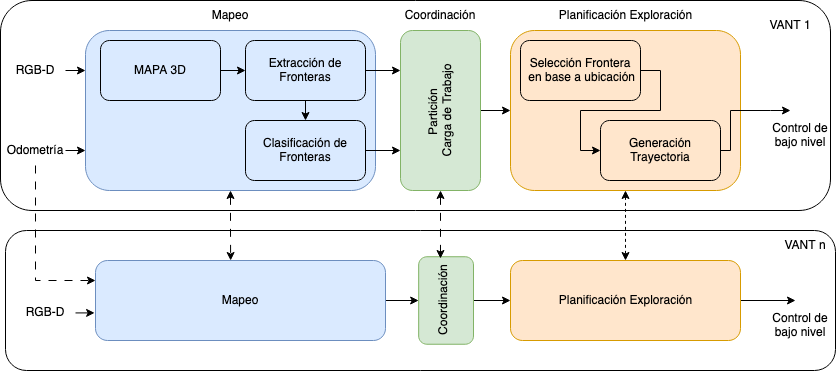
\includegraphics[width=0.5\textwidth]{arqui_drone}
\caption{Extensión Multi-VANT, La arquitectura multi-VANT propuesta se centra en tres elementos principales creación de un mapa, coordinación, planificación de exploración}
\label{fig:multivant}
\end{figure}

\begin{itemize}
\item Construcción de la representación del ambiente (Mapa)
\item Coordinación y reparto de carga de trabajo
\item Exploración
\item Comunicación
\end{itemize}

Para nuestra estrategia, tomaremos un enfoque basado en algoritmos de búsqueda. Por su rápidez y su generación de trayectorias casi-óptimas cuando son guiadas con una heurística. También han demostrado resolver un replanteamiento en base a un cambio en sus objetivos como son el caso de algoritmos como D*-Lite \cite{D_estrella}.\\

Un planificador global encontrará una ruta en base a las fronteras detectadas que será asignada a los VANTS disponibles en la tarea de exploración.\\

Para conservar una autonomía en la navegación y reducir los riesgos de colisión, se hará uso de un planificador local. Este será el encargado de generar una ruta libre de colisiones. Existen diversos enfoques en la construcción de un planificador local, estos planificadores pueden presentar comportamientos reactivos, aprendizaje máquina o leyes de control que guíen su trayectoria. Un planificador local es rico en información que a su vez es usada en la planificación global. Ese conocimiento incluye la información de los sensores, que son de ayuda en la construcción y mantenimiento de un mapa. Nuestro enfoque busca contar un comportamiento reactivo que le permita al VANT evitar oportunamente obstáculos a su paso.\\

Con ayuda de un mapa que represente la información de obstáculos recolectados con ayuda de sensores de tipo láser o cámaras con tecnología RGB-D, se logrará tener una representación del ambiente que será de ayuda para la planificación de trayectorias para los múltiples VANTS. Un enfoque con Voxel, ayuda a tener una representación en tres dimensiones. Con el uso de una cuadrícula de voxels el ambiente puede ser representado en base a un enfoque probabilístico, indicando la probabilidad de que un espacio pueda estar o no ocupado.\\

Debido a que contamos con un ambiente en tres dimensiones, su representación es computacionalmente costosa y requiere el uso de una estructura de datos que permita la ejecución de múltiples búsquedas al mismo tiempo. Al agregar información relacionada a las lecturas provenientes de los valores de los sensores y una política de actualización en base al tiempo de lectura, nos ayudará a mantener un mapa actualizado.\\

Como se ha mencionado, la autonomía de vuelo puede ser realizada combinando el control de vuelo, planificación de trayectorias, navegación y evasión de obstáculos.\\

En sistemas de vuelo autónomo, la toma de decisiones determinará las instrucciones de vuelo en base a una tarea. Como un primer alcance de exploración coordinada, se explorará la estrategia propuesta por \citeauthor{CINVESTAM2013} \cite{CINVESTAM2013}, que logra un funcionamiento asincróno manteniendo una cohesión entre los robots ayudando en tener una comunicación entre ellos, además la estrategia de coordinación permite incluir nuevos miembros a la exploración contando con una versión actual del estado de la exploración.\\

La repartición de fronteras pretende tomar en consideración la cercanía con el robot más cercano, si el objetivo es descubierto por otro VANT, se considerá una señal de parada y obligarlo a reiniciar un proceso de oferta para seleccionar un nuevo objetivo.\\

En paralelo, un módulo de comunicación y recepción de mensajes maneja la información de los miembros del equipo.\\

El mecanismo de auto-ofertas, el sensado y construcción del mapa se llevan a cabo continuamente durante el proceso de navegación.\\

Aunque el resultado esperado en robótica es probarse de manera real, existen muchos simuladores que han demostrado buenos desempeños, la existencia de diversos simuladores (Gazebo, Microsoft AirSim, Webots) \cite{Chen2023}, validan el uso extenso de ellos en el desarrollo tecnológico.\\

La arquitectura propuesta se validará haciendo uso del middleware ROS (Robot Operating System) y Gazebo implicando el desarrollo de un sistema colaborativo. En esta configuración, los múltiples VANTS se comunican e interactúan en tiempo real a través de ROS, aprovechando sus nodos de comunicación y control. Gazebo, por su parte, proporciona un entorno de simulación realista que permite probar y validar algoritmos de exploración en un ambiente tridimensional y dinámico. Los modelos virtuales de los VANTs en Gazebo, sincronizados con los nodos de control en ROS, permiten evaluar los algoritmos de planificación de rutas, control de colisiones y toma de decisiones en un escenario simulado antes de su implementación en entornos del mundo real. %Esta integración de ROS y Gazebo en la exploración coordinada multi-VANT ofrece un marco sólido para el desarrollo, pruebas y refinamiento de estrategias de exploración que pueden ser aplicadas en aplicaciones diversas, desde la vigilancia y la búsqueda y rescate hasta la inspección de infraestructuras críticas.

\section{Resultados Esperados y Análisis}

%La implementación y evaluación exitosa de la propuesta.
Se espera que los algoritmos de coordinación en tareas de exploración de múltiples VANTS produzcan mejoras significativas en la eficiencia, cobertura y adaptabilidad de la exploración. El siguiente análisis proporciona una visión general de los resultados esperados y sus implicaciones.

\subsection*{Porcentaje de cobertura de exploración}

Una de las principales métricas de desempeño es el porcentaje de cobertura de exploración, que representa la proporción del área de exploración cubierta con éxito por el sistema multi-VANTS. Se prevé que la aplicación de algoritmos de coordinación avanzados, conducirá a un aumento notable en el porcentaje de cobertura.

\begin{itemize}
\item Análisis comparativo de la cobertura alcanzada por los algoritmos de coordinación propuestos frente a los enfoques en el estado del arte.
\item Prueba de la adaptabilidad a terrenos variables y dinámicos.
\item Identificación de áreas con mejor cobertura debido a los mecanismos de priorización.
\end{itemize}
  
\subsection*{Utilización y eficiencia de recursos}

La utilización eficiente de los recursos es crucial en las tareas de exploración de múltiples VANTS para extender la duración de la misión y optimizar la recopilación de datos. Los resultados esperados se centrarán en la utilización de recursos, incluida la energía, el tiempo de los sensores y el almacenamiento de datos.

\begin{itemize}
\item Evaluación comparativa del consumo de recursos entre algoritmos de coordinación avanzados y métodos tradicionales.
  
\item Evaluación de la adaptabilidad de algoritmos a diferentes limitaciones de recursos y objetivos de misión.
  
\item Identificación de la estrategia eficiente en el uso de recursos que prolonguen la duración de la misión y la calidad de los datos al mismo tiempo que conservan la energía y el almacenamiento.
  
\end{itemize}

\subsection*{Toma de decisiones en tiempo real y evasión de obstáculos}

Los sistemas multi-VANT a menudo enfrentan desafíos a la hora de tomar decisiones en tiempo real, como evitar obstáculos y planificar rutas. Se espera que las solución propuesta muestre capacidades de toma de decisiones.

\begin{itemize}
\item Análisis comparativo de la velocidad y eficiencia en la toma de decisiones entre algoritmos avanzados y enfoques tradicionales.
\item Evaluación de mecanismos de evasión de obstáculos en tiempo real, especialmente en entornos no estructurados e impredecibles.
\end{itemize}

El examen de los resultados esperados permitirá evaluar la efectividad y la viabilidad práctica de los algoritmos de coordinación propuestos en las tareas de exploración de múltiples VANTS. Los descubrimientos proporcionarán fundamentos para mejoras y usos adicionales en contextos de exploración con múltiples VANTS.

\section{Conclusiones}

En conclusión, la incesante expansión de la tecnología de los vehículos aéreos no tripulados (VANTS) está brindando a la humanidad oportunidades incomparables para utilizarlos en tareas de exploración y vigilancia. Nuestro artículo busca ampliar el creciente cuerpo de conocimientos mediante la investigación de estrategias para la coordinación de múltiples VANTS en tareas de exploración. A través de marcos teóricos, diseño de algoritmos y metodologías propuestas, aspiramos a allanar el camino para avances innovadores en este campo. Al fomentar la innovación en la coordinación de múltiples VANTS, esperamos contribuir a la transformación de las industrias y el avance de la comprensión científica.\\

Los resultados y análisis esperados indican las perspectivas prometedoras de esta estrategia, incluyendo mayores niveles de cobertura y una utilización eficiente de los recursos. Aunque existen desafíos y limitaciones inherentes a las complejidades de las tareas reales de exploración, abordar estos desafíos es una tarea continua para la comunidad investigadora, brindando una dirección clara para futuras mejoras y adaptaciones.\\

%En conclusión, este artículo destaca que el potencial de las estrategias de coordinación de múltiples VANTS es ilimitado. Prometen redefinir la forma en que exploramos, monitoreamos y respondemos a diversos entornos y situaciones de desastre. Las estrategias presentadas no son solo conceptos teóricos, son invitaciones a hacer que la exploración sea más eficiente, adaptable y significativa.\\

%Como investigadores, ingenieros y exploradores, nos encontramos en el umbral de una nueva era en las tareas de exploración automática. Estas estrategias son herramientas en nuestras manos, listas para moldear el futuro de la exploración. A través de la investigación, la experimentación y el compromiso constante para superar los desafíos, podemos garantizar que la coordinación de múltiples VANTS juegue un papel fundamental en abordar los problemas más urgentes del mundo.

%\section*{Agradecimientos}
%Incluir fuentes de financiamiento u otro apoyo para la realización del proyecto (No. proyecto, Fondo, becas, etc). Se pueden incluir agradecimientos a personas o grupos estrechamente relacionados con el trabajo presentado en el artículo.

%% incluya la bibliografía en un archivo separado .bib

\setcitestyle{numbers}
\bibliographystyle{unsrtnat}%{plainnat}%{abbrvnat}
\bibliography{samplebib}

%\bibliographystyle{ACM-Reference-Format}
%\bibliographystyle{unsrt}
%\bibliography{samplebib}


\end{document}
\endinput
%%
%%
